\documentclass[a4paper]{article}

\def\npart {III}
\def\nterm {Michaelmas}
\def\nyear {2017}
\def\nlecturer {C.\ P.\ Caulfield}
\def\ncourse {Hydrodynamic Stability}

% Imports
\ifx \nextra \undefined
  \usepackage[pdftex,
    hidelinks,
    pdfauthor={Dexter Chua},
    pdfsubject={Cambridge Maths Notes: Part \npart\ - \ncourse},
    pdftitle={Part \npart\ - \ncourse},
  pdfkeywords={Cambridge Mathematics Maths Math \npart\ \nterm\ \nyear\ \ncourse}]{hyperref}
  \title{Part \npart\ - \ncourse}
\else
  \usepackage[pdftex,
    hidelinks,
    pdfauthor={Dexter Chua},
    pdfsubject={Cambridge Maths Notes: Part \npart\ - \ncourse\ (\nextra)},
    pdftitle={Part \npart\ - \ncourse\ (\nextra)},
  pdfkeywords={Cambridge Mathematics Maths Math \npart\ \nterm\ \nyear\ \ncourse\ \nextra}]{hyperref}

  \title{Part \npart\ - \ncourse \\ {\Large \nextra}}
\fi

\author{Lectured by \nlecturer \\\small Notes taken by Dexter Chua}
\date{\nterm\ \nyear}

\usepackage{alltt}
\usepackage{amsfonts}
\usepackage{amsmath}
\usepackage{amssymb}
\usepackage{amsthm}
\usepackage{booktabs}
\usepackage{caption}
\usepackage{enumitem}
\usepackage{fancyhdr}
\usepackage{graphicx}
\usepackage{mathtools}
\usepackage{microtype}
\usepackage{multirow}
\usepackage{pdflscape}
\usepackage{pgfplots}
\usepackage{siunitx}
\usepackage{tabularx}
\usepackage{tikz}
\usepackage{tkz-euclide}
\usepackage[normalem]{ulem}
\usepackage[all]{xy}

\pgfplotsset{compat=1.12}

\pagestyle{fancyplain}
\lhead{\emph{\nouppercase{\leftmark}}}
\ifx \nextra \undefined
  \rhead{
    \ifnum\thepage=1
    \else
      \npart\ \ncourse
    \fi}
\else
  \rhead{
    \ifnum\thepage=1
    \else
      \npart\ \ncourse\ (\nextra)
    \fi}
\fi
\usetikzlibrary{arrows}
\usetikzlibrary{decorations.markings}
\usetikzlibrary{decorations.pathmorphing}
\usetikzlibrary{positioning}
\usetikzlibrary{fadings}
\usetikzlibrary{intersections}
\usetikzlibrary{cd}

\newcommand*{\Cdot}{\raisebox{-0.25ex}{\scalebox{1.5}{$\cdot$}}}
\newcommand {\pd}[2][ ]{
  \ifx #1 { }
    \frac{\partial}{\partial #2}
  \else
    \frac{\partial^{#1}}{\partial #2^{#1}}
  \fi
}

% Theorems
\theoremstyle{definition}
\newtheorem*{aim}{Aim}
\newtheorem*{axiom}{Axiom}
\newtheorem*{claim}{Claim}
\newtheorem*{cor}{Corollary}
\newtheorem*{defi}{Definition}
\newtheorem*{eg}{Example}
\newtheorem*{fact}{Fact}
\newtheorem*{law}{Law}
\newtheorem*{lemma}{Lemma}
\newtheorem*{notation}{Notation}
\newtheorem*{prop}{Proposition}
\newtheorem*{thm}{Theorem}

\renewcommand{\labelitemi}{--}
\renewcommand{\labelitemii}{$\circ$}
\renewcommand{\labelenumi}{(\roman{*})}

\let\stdsection\section
\renewcommand\section{\newpage\stdsection}

% Strike through
\def\st{\bgroup \ULdepth=-.55ex \ULset}

% Maths symbols
\newcommand{\bra}{\langle}
\newcommand{\ket}{\rangle}

\newcommand{\N}{\mathbb{N}}
\newcommand{\Z}{\mathbb{Z}}
\newcommand{\Q}{\mathbb{Q}}
\renewcommand{\H}{\mathbb{H}}
\newcommand{\R}{\mathbb{R}}
\newcommand{\C}{\mathbb{C}}
\newcommand{\Prob}{\mathbb{P}}
\renewcommand{\P}{\mathbb{P}}
\newcommand{\E}{\mathbb{E}}
\newcommand{\F}{\mathbb{F}}
\newcommand{\cU}{\mathcal{U}}
\newcommand{\RP}{\mathbb{RP}}
\newcommand{\CP}{\mathbb{CP}}

\newcommand{\ph}{\,\cdot\,}

\DeclareMathOperator{\sech}{sech}
\DeclareMathOperator{\cosech}{cosech}
\DeclareMathOperator{\cosec}{cosec}

\DeclareMathOperator{\covol}{covol}
\DeclareMathOperator{\vol}{vol}

\let\Im\relax
\let\Re\relax
\DeclareMathOperator{\Im}{Im}
\DeclareMathOperator{\Re}{Re}
\DeclareMathOperator{\im}{im}
\DeclareMathOperator{\image}{image}
\DeclareMathOperator{\Ann}{Ann}

\DeclareMathOperator*{\res}{res}
\DeclareMathOperator{\Res}{Res}
\DeclareMathOperator{\Ind}{Ind}

\DeclareMathOperator{\tr}{tr}
\DeclareMathOperator{\diag}{diag}
\DeclareMathOperator{\rank}{rank}
\DeclareMathOperator{\card}{card}
\DeclareMathOperator{\spn}{span}
\DeclareMathOperator{\adj}{adj}

\DeclareMathOperator{\erf}{erf}
\DeclareMathOperator{\erfc}{erfc}

\DeclareMathOperator{\ord}{ord}
\DeclareMathOperator{\Sym}{Sym}

\DeclareMathOperator{\sgn}{sgn}
\DeclareMathOperator{\orb}{orb}
\DeclareMathOperator{\stab}{stab}
\DeclareMathOperator{\ccl}{ccl}

\DeclareMathOperator{\lcm}{lcm}
\DeclareMathOperator{\hcf}{hcf}

\DeclareMathOperator{\Int}{Int}
\DeclareMathOperator{\id}{id}

\DeclareMathOperator{\betaD}{beta}
\DeclareMathOperator{\gammaD}{gamma}
\DeclareMathOperator{\Poisson}{Poisson}
\DeclareMathOperator{\binomial}{binomial}
\DeclareMathOperator{\multinomial}{multinomial}
\DeclareMathOperator{\Bernoulli}{Bernoulli}
\DeclareMathOperator{\like}{like}

\DeclareMathOperator{\var}{var}
\DeclareMathOperator{\cov}{cov}
\DeclareMathOperator{\bias}{bias}
\DeclareMathOperator{\mse}{mse}
\DeclareMathOperator{\corr}{corr}

\DeclareMathOperator{\otp}{otp}
\DeclareMathOperator{\dom}{dom}

\DeclareMathOperator{\Root}{Root}
\DeclareMathOperator{\supp}{supp}
\DeclareMathOperator{\rel}{rel}
\DeclareMathOperator{\Hom}{Hom}
\DeclareMathOperator{\Aut}{Aut}
\DeclareMathOperator{\Gal}{Gal}
\DeclareMathOperator{\Mat}{Mat}
\DeclareMathOperator{\End}{End}
\DeclareMathOperator{\Char}{char}
\DeclareMathOperator{\ev}{ev}
\DeclareMathOperator{\St}{St}
\DeclareMathOperator{\Lk}{Lk}
\DeclareMathOperator{\disc}{disc}
\DeclareMathOperator{\Isom}{Isom}
\DeclareMathOperator{\length}{length}
\DeclareMathOperator{\energy}{energy}
\DeclareMathOperator{\area}{area}
\DeclareMathOperator{\Syl}{Syl}
\DeclareMathOperator{\cl}{cl}
\DeclareMathOperator{\fix}{fix}

\newcommand{\GL}{\mathrm{GL}}
\newcommand{\SL}{\mathrm{SL}}
\newcommand{\PGL}{\mathrm{PGL}}
\newcommand{\PSL}{\mathrm{PSL}}
\newcommand{\PSU}{\mathrm{PSU}}
\newcommand{\Or}{\mathrm{O}}
\newcommand{\SO}{\mathrm{SO}}
\newcommand{\U}{\mathrm{U}}
\newcommand{\SU}{\mathrm{SU}}

\renewcommand{\d}{\mathrm{d}}
\newcommand{\D}{\mathrm{D}}

\tikzset{->/.style = {decoration={markings,
                                  mark=at position 1 with {\arrow[scale=2]{latex'}}},
                      postaction={decorate}}}
\tikzset{<-/.style = {decoration={markings,
                                  mark=at position 0 with {\arrowreversed[scale=2]{latex'}}},
                      postaction={decorate}}}
\tikzset{<->/.style = {decoration={markings,
                                   mark=at position 0 with {\arrowreversed[scale=2]{latex'}},
                                   mark=at position 1 with {\arrow[scale=2]{latex'}}},
                       postaction={decorate}}}
\tikzset{->-/.style = {decoration={markings,
                                   mark=at position #1 with {\arrow[scale=2]{latex'}}},
                       postaction={decorate}}}
\tikzset{-<-/.style = {decoration={markings,
                                   mark=at position #1 with {\arrowreversed[scale=2]{latex'}}},
                       postaction={decorate}}}

\tikzset{circ/.style = {fill, circle, inner sep = 0, minimum size = 3}}
\tikzset{mstate/.style={circle, draw, blue, text=black, minimum width=0.7cm}}

\definecolor{mblue}{rgb}{0.2, 0.3, 0.8}
\definecolor{morange}{rgb}{1, 0.5, 0}
\definecolor{mgreen}{rgb}{0.1, 0.4, 0.2}
\definecolor{mred}{rgb}{0.5, 0, 0}

\def\drawcirculararc(#1,#2)(#3,#4)(#5,#6){%
    \pgfmathsetmacro\cA{(#1*#1+#2*#2-#3*#3-#4*#4)/2}%
    \pgfmathsetmacro\cB{(#1*#1+#2*#2-#5*#5-#6*#6)/2}%
    \pgfmathsetmacro\cy{(\cB*(#1-#3)-\cA*(#1-#5))/%
                        ((#2-#6)*(#1-#3)-(#2-#4)*(#1-#5))}%
    \pgfmathsetmacro\cx{(\cA-\cy*(#2-#4))/(#1-#3)}%
    \pgfmathsetmacro\cr{sqrt((#1-\cx)*(#1-\cx)+(#2-\cy)*(#2-\cy))}%
    \pgfmathsetmacro\cA{atan2(#2-\cy,#1-\cx)}%
    \pgfmathsetmacro\cB{atan2(#6-\cy,#5-\cx)}%
    \pgfmathparse{\cB<\cA}%
    \ifnum\pgfmathresult=1
        \pgfmathsetmacro\cB{\cB+360}%
    \fi
    \draw (#1,#2) arc (\cA:\cB:\cr);%
}
\newcommand\getCoord[3]{\newdimen{#1}\newdimen{#2}\pgfextractx{#1}{\pgfpointanchor{#3}{center}}\pgfextracty{#2}{\pgfpointanchor{#3}{center}}}

\def\Xint#1{\mathchoice
   {\XXint\displaystyle\textstyle{#1}}%
   {\XXint\textstyle\scriptstyle{#1}}%
   {\XXint\scriptstyle\scriptscriptstyle{#1}}%
   {\XXint\scriptscriptstyle\scriptscriptstyle{#1}}%
   \!\int}
\def\XXint#1#2#3{{\setbox0=\hbox{$#1{#2#3}{\int}$}
     \vcenter{\hbox{$#2#3$}}\kern-.5\wd0}}
\def\ddashint{\Xint=}
\def\dashint{\Xint-}


\newcommand\Ra{\mathrm{Ra}}
\renewcommand\Pr{\mathrm{Pr}}
\begin{document}
\maketitle
{\small
\setlength{\parindent}{0em}
\setlength{\parskip}{1em}
Developing an understanding by which ``small'' perturbations grow, saturate and modify fluid flows is central to addressing many challenges of interest in fluid mechanics. Furthermore, many applied mathematical tools of much broader relevance have been developed to solve hydrodynamic stability problems, and hydrodynamic stability theory remains an exceptionally active area of research, with several exciting new developments being reported over the last few years.

In this course, an overview of some of these recent developments will be presented. After an introduction to the general concepts of flow instability, presenting a range of examples, the major content of this course will be focussed on the broad class of flow instabilities where velocity ``shear'' and fluid inertia play key dynamical roles. Such flows, typically characterised by sufficiently“high” Reynolds number $Ud/\nu$, where $U$ and $d$ are characteristic velocity and length scales of the flow, and $\nu$ is the kinematic viscosity of the fluid, are central to modelling flows in the environment and industry. They typically demonstrate the key role played by the redistribution of vorticity within the flow, and such vortical flow instabilities often trigger the complex, yet hugely important process of ``transition to turbulence''.

A hierarchy of mathematical approaches will be discussed to address a range of ``stability'' problems, from more traditional concepts of ``linear'' infinitesimal normal mode perturbation energy growth on laminar parallel shear flows to transient, inherently nonlinear perturbation growth of general measures of perturbation magnitude over finite time horizons where flow geometry and/or fluid properties play a dominant role. The course will also discuss in detail physical interpretations of the various flow instabilities considered, as well as the industrial and environmental application of the results of the presented mathematical analyses

\subsubsection*{Pre-requisites}
Elementary concepts from undergraduate real analysis. Some knowledge of complex analysis would be advantageous (e.g.\ the level of IB Complex Analysis/Methods). No knowledge of functional analysis is assumed.
}
\tableofcontents

\section{Instability of fluid at rest}
\subsection{Rayleigh--Taylor instability}
In this section, we would like to investigate the stability of a surface between two fluids:
\begin{center}
  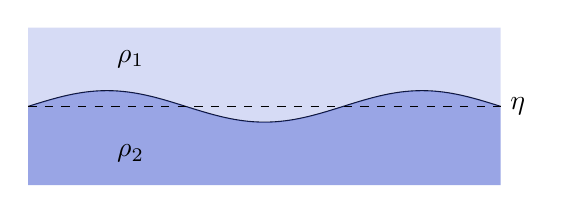
\begin{tikzpicture}
    \draw (-3, 0) sin (-2, 0.2) cos (-1, 0) sin (0, -0.2) cos (1, 0) sin (2, 0.2) cos (3, 0) node [right] {$\eta$};
    \fill [mblue, opacity=0.5] (-3, -1) -- (-3, 0) sin (-2, 0.2) cos (-1, 0) sin (0, -0.2) cos (1, 0) sin (2, 0.2) cos (3, 0) -- (3, -1);
    \fill [mblue, opacity=0.2] (-3, 1) -- (-3, 0) sin (-2, 0.2) cos (-1, 0) sin (0, -0.2) cos (1, 0) sin (2, 0.2) cos (3, 0) -- (3, 1);

    \draw [dashed] (-3, 0) -- (3, 0);
    \node at (-1.7, -0.6) {$\rho_2$};
    \node at (-1.7, 0.6) {$\rho_1$};
  \end{tikzpicture}
\end{center}
We assume the two fluids have densities $\rho_1$ and $\rho_2$, and are separated by a smooth interface parametrized by the deviation $\eta$. 

Recall that the Navier--Stokes equations for an incompressible fluid are
\[
  \rho\left(\frac{\partial \mathbf{u}}{\partial t} + \mathbf{u} \cdot \nabla \mathbf{u}\right) = - \nabla P- g \rho \hat{\mathbf{z}} + \mu \nabla^2 \mathbf{u},\quad \nabla \cdot \mathbf{u} = 0.
\]
Usually, when doing fluid mechanics, we assume density is constant, and divide the whole equation across by $\rho$. We can then forget the existence of $\rho$ and carry on. We can also get rid of the gravity term. We know that the force of gravity is balanced out by a hydrostatic pressure gradient. More precisely, we can write
\[
  P = P_h(z) + p (x, t),
\]
where $P_h$ satisfies
\[
  \frac{\partial P_h}{\partial z} = -g\rho.
\]
We can then write our equation as
\[
  \frac{\partial \mathbf{u}}{\partial t} + \mathbf{u}\cdot \nabla \mathbf{u} = - \nabla \left(\frac{p}{\rho}\right) + \nu \nabla^2 \mathbf{u}.
\]
To do all of these, we must assume that the density $\rho$ is constant, but this is clearly not the case when we have tow distinct fluids.

Since it is rather difficult to move forward without making \emph{any} simplifying assumptions, we shall focus on the case of inviscid fluids, so that we take $\nu = 0$. We will also assume that the fluid is irrotational. In this case, it is convenient to use the vector calculus identity
\[
  \mathbf{u} \cdot \nabla \mathbf{u} = \nabla \left(\frac{1}{2}|\mathbf{u}|^2\right) - \mathbf{u} \times (\nabla \times \mathbf{u}),
\]
where we can now drop the second term. Moreover, since $\nabla \times \mathbf{u} = 0$, Stokes' theorem allows us to write $\mathbf{u} = \nabla \phi$ for some \term{velocity potential} $\phi$. Finally, in each separate region, the density $\rho$ is constant. So we can now write
\[
  \nabla \left(\rho \frac{\partial \phi}{\partial t} + \frac{1}{2} \rho |\nabla \phi|^2 + P + g \rho z\right) = 0.
\]
This is \term{Bernoulli's theorem}.

Applying these to our scenario, since we have two fluids, we have two separate velocity potentials $\phi_1, \phi_2$ for the two two regions. Both of these independently satisfy the incompressibility hypothesis
\[
  \nabla^2\phi_{1, 2} = 0.
\]
Bernoulli's theorem tells us the quantity
\[
  \rho \frac{\partial \phi}{\partial t} + \frac{1}{2} \rho |\nabla \phi|^2 + P + g \rho z
\]
should be constant across the fluid. Our investigation will not use the full equation. All we will need is that this quantity matches at the interface, so that we have
\[
  \left.\rho_1 \frac{\partial \phi_1}{\partial t} + \frac{1}{2} \rho_1 |\nabla \phi_1|^2 + P_1 + g \rho_1 \eta\right|_{z = \eta} = \left.\rho_2 \frac{\partial \phi_2}{\partial t} + \frac{2}{2} \rho_2 |\nabla \phi_2|^2 + P_2 + g \rho_2 \eta\right|_{z = \eta}.
\]
To understand the interface, we must impose boundary conditions. First of all the vertical velocities of the fluids must match with the interface, so we impose the \term{kinematic boundary condition}
\[
  \left.\frac{\partial \phi_1}{\partial z} \right|_{z = \eta} = \left.\frac{\partial \phi_2}{\partial z} \right|_{z = \eta} = \frac{\D \eta}{\D t},
\]
where
\[
  \D = \frac{\partial}{\partial t} + \mathbf{u} \cdot \nabla
\]
We also make another, perhaps dubious boundary condition, namely that the pressure is continuous along the interface. This does not hold at all interfaces. For example, if we have a balloon, then the pressure inside is greater than the pressure outside, since that is what holds the balloon up. In this case, it is the rubber that is exerting a force to maintain the pressure difference. In our case, we only have two fluids meeting, and there is no reason to assume a discontinuity in pressure, and thus we shall assume it is continuous. If you are not convinced, this is good, and we shall later see this is indeed a dubious assumption.

But assuming it for the moment, this allows us to simplify our Bernoulli's theorem to give
\[
  \rho_1 \frac{\partial \phi_1}{\partial t} + \frac{1}{2} \rho_1 |\nabla \phi_1|^2 + g \rho_1 \eta = \rho_2 \frac{\partial \phi_2}{\partial t} + \frac{2}{2} \rho_2 |\nabla \phi_2|^2 + g \rho_2 \eta.
\]
There is a final boundary condition that is specific to our model. What we are going to do is that we will start with a flat, static solution with $\mathbf{u} = 0$ and $\eta = 0$. We then perturb $\eta$ a bit, and see what happens to our fluid. In particular, we want to see if the perturbation is stable.

Since we expect the interesting behaviour to occur only near the interface, we make the assumption that there is no velocity in the far field, i.e.\ $\phi_1 \to 0$ as $z \to \infty$ and $\phi_2 \to 0$ as $z \to-\infty$ (and similarly for the derivatives). For simplicity, we also assume there is no $y$ dependence.

We now have equations and boundary conditions, so we can solve them. But these equations are pretty nasty and non-linear. At this point, one sensible approach is to linearize the equations by assuming everything is small. In addition to assuming that $\eta$ is small, we also need to assume that various derivatives such as $\nabla \phi$ are small, so that we can drop all second-order terms. Since $\eta$ is small, the value of, say, $\frac{\partial \phi_1}{\partial z}$ at $\eta$ should be similar to that at $\eta = 0$. Since $\frac{\partial \phi_1}{\partial z}$ itself is already assumed to be small, the difference would be second order in smallness.

So we replace all evaluations at $\eta$ with evaluations at $z = 0$. We are then left with the collection of $3$ equations
\begin{align*}
  \nabla^2 \phi_{1, 2} &= 0\\
  \left.\frac{\partial \phi_{1, 2}}{\partial z}\right|_{z = 0} &= \eta_t\\
  \left.\rho_1 \frac{\partial \phi_1}{\partial t} + g \rho_1 \eta \right|_{z = 0} &= \left.\rho_2 \frac{\partial \phi_2}{\partial t} + g \rho_2 \eta \right|_{z = 0}.
\end{align*}

This is a nice linear problem, and we can analyze the Fourier modes of the solutions. We plug in an ansatz
\begin{align*}
  \phi_{1, 2}(x, z, t) &= \hat{\phi}_{1, 2}(z) e^{i(kx - \omega t)}\\
  \eta(x, t) &= B e^{i(kx - \omega t)}.
\end{align*}
Substituting into Laplace's equation gives
\[
  \hat{\phi}_{1, 2} - k^2 \hat{\phi}_{1, 2} = 0.
\]
Using the far field boundary conditions, we see that we have a family of solutions
\[
  \hat{\phi}_1 = A_1 e^{-kz},\quad \hat{\phi}_2 = A_2 e^{kz}.
\]
The kinematic boundary condition tells us we must have
\[
  \hat{\phi}_{1, 2}'(0) = -i\omega B.
\]
We can solve this to get
\[
  B = \frac{k A_1}{i \omega} = - \frac{kA_2}{ i \omega}.
\]
In particular, we must have $A \equiv A_1 = - A_2$. We can then write
\[
  \eta = \frac{kA}{i\omega} e^{ik(kx - \omega t)}.
\]
Plugging these into the final equation gives us
\[
  \rho_1 (-i\omega A) + g \rho_1 \frac{k A}{i \omega} = \rho_2 i \omega A + g \rho_2 \frac{kA}{i \omega}.
\]
Crucially, we can cancel the $A$ throughout the equation, and gives us a result independent of $A$. This is, after all, the point of linearization. Solving this gives us a \term{dispersion relation} relating the frequency (or phase speed $c_p = \omega/k$) to the wavenumber:
\[
  \omega^2 = \frac{g(\rho_2 - \rho_1)k}{\rho_1 + \rho_2}.
\]
If $\rho_2 \gg \rho_1$, then this reduces to $\omega^2 \approx gk$, and this is the usual dispersion relation for deep water waves. On the other hand, if $\rho_2 - \rho_1 > 0$ is small, this can lead to waves of rather low frequency, which is something we can observe in cocktails, apparently.

But nothing in our analysis actually required $\rho_2 > \rho_1$. Suppose we had $\rho_1 > \rho_2$. This amounts to putting the heavier fluid on top of the lighter one. Anyone who has tried to turn a cup of water upside down will know this is highly unstable. Can we see this from our analysis?

If $\rho_1 < \rho_2$, then $\omega$ has to be imaginary. We shall write it as $\omega = \pm i \sigma$, where $\sigma > 0$. We can then compute
\[
  \sigma = \sqrt{\frac{g(\rho_1 - \rho_2)k}{\rho_1 + \rho_2}}.
\]
Writing out our expression for $\phi_{1, 2}$, we see that there are $e^{\pm \sigma t}$ terms, and the $e^{\sigma t}$ term dominates in the long run, causing $\phi_{1, 2}$ to grow exponentially. This is the \emph{Rayleigh--Taylor instability}.

There is more to say about the instability. As the wavelength decreases, $k$ increases, and we see that $\sigma$ increases as well. Thus, we see that short-scale perturbations blow up exponentially much more quickly, which means the system is not very well-posed. This is the \term{ultra-violet catastrophe}. Of course, we should not trust our model here. Recall that in our simplifying assumptions, we not only assumed that the amplitudes of our $\phi$ and $\eta$ were small, but also that their derivatives were small. The large $k$ behaviour gives us large $x$ derivatives, and so we have to take into account the higher order terms as well.

But we can also provide physical reasons for why small scales perturbations should be suppressed by such a system. In our model, we assumed there is no surface tension. Surface tension quantifies the tendency of interfaces between fluids to minimize surface area. We know that small-scale variations will cause a large surface area, and so the surface tension will suppress these variations. Mathematically, what the surface allows for is a pressure jump across the interface.

Surface tension is quantified by $\gamma$, the force per unit length. This has dimensions $[\gamma] = MT^{-1}$. Empirically, we observe that the pressure difference across the interface is
\[
  \Delta p = - \gamma \nabla \cdot \hat{\mathbf{n}} = 2 \gamma H = \gamma \left(\frac{1}{R_x} + \frac{1}{R_y}\right),
\]
where $\hat{\mathbf{n}}$ is the unit normal and $H$ is the \term{mean curvature}. This is an empirical result.

Again, we assume no dependence in the $y$ direction, so we have a cylindrical interface with a single radius of curvature. Linearizing, we have a pressure difference of
\[
  (P_2 - P_1) |_{z = \eta} = \frac{\gamma}{R_x} = - \gamma \frac{\frac{\partial^2 \eta}{\partial x^2}}{\left(1 + \left(\frac{\partial \eta}{\partial x}\right)^2\right)^{3/2}} \approx -\gamma \frac{\partial^2 \eta}{\partial x^2}.
\]
Therefore the (linearized) dynamic boundary condition becomes
\[
  \left.\rho_1 \frac{\partial \phi_1}{\partial t} + g \rho_1 \eta\right|_{z =0 } + \gamma \frac{\partial^2 \eta}{\partial x^2} = \left. \rho_2 \frac{\partial \phi_2}{\partial t} + g \rho_2 \eta\right|_{z = 0}.
\]
If we run the previous analysis again, we find a dispersion relation of
\[
  \omega^2 = \frac{g(\rho_2 - \rho_1)k + \gamma k^3}{\rho_1 + \rho_2}.
\]
Since $\gamma$ is always positive, even if we are in the situation when $\rho_1 > \rho_2$, for $k$ sufficiently large, the system is stable. Of course, for small $k$, the system is still unstable --- we still expect water to fall out even with surface tension. In the case $\rho_1 < \rho_2$, what we get is known as \term{internal gravity-capillary waves}.

In the unstable case, we have
\[
  \sigma^2 = k \left(\frac{g(\rho_2 - \rho_1)}{\rho_1 + \rho_2}\right) (1 - l_c^2 k^2),
\]
where
\[
  l_c^2 = \frac{\gamma}{g (\rho_1 - \rho_2)}
\]
is a characteristic length scale. For $k \ell_c > 1$, the oscillations are stable, and the maximum value of $k$ is attained at $k = \frac{l_c}{\sqrt{3}}$.
% insert plot

In summary, we have a range of wavelength, and we have identified a ``most unstable wavelength''. Over time, if all frequencies modes are triggered, we should expect this most unstable wavelength to dominate. But it is rather hopeful thinking, because this is the result of linear analysis, and we can't expect it to carry on to the non-linear regime.

\subsection{Rayleigh--B\'enard convection}
The next system we want to study is something that looks like this:
\begin{center}
  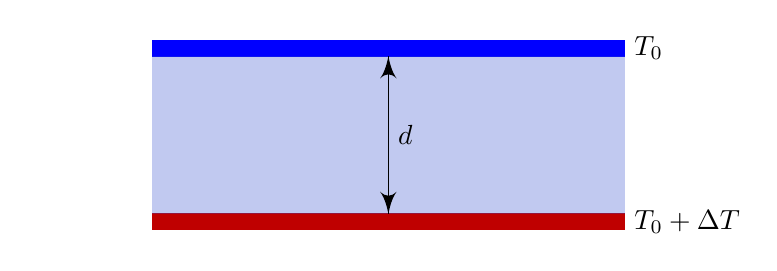
\begin{tikzpicture}
    \draw [red!50!mred, fill] (0, 0) rectangle (6, -0.2);
    \draw [blue, fill] (0, 2) rectangle (6, 2.2);

    \fill [mblue, opacity=0.3] (0, 0) rectangle (6, 2);

    \node [right] at (6, 2.1) {$T_0$};
    \node [right] at (6, -0.1) {$T_0 + \Delta T$};
    \node [white, left] at (0, -0.1) {$T_0 + \Delta T$};

    \draw [<->] (3, 0) -- (3, 2) node [pos=0.5, right] {$d$};
  \end{tikzpicture}
\end{center}
There is a hot plate at the bottom, a cold plate on top, and some fluid in between. We would naturally expect heat to transmit from the bottom to the top. There are two ways this can happen:
\begin{itemize}
  \item Conduction: Heat simply diffuses from the bottom to the top, without any fluid motion.
  \item Convection: The fluid at the bottom heats up, expands, becomes lighter, and moves to the top.
\end{itemize}
The first factor is controlled purely by thermal diffusivity $\kappa$, while the latter is mostly controlled by the viscosity $\nu$. It is natural to expect that when the temperature gradient $\Delta T$ is small, most of the heat transfer is due to conduction, as there isn't enough force to overcome the viscosity to move fluid around. When $\Delta T$ is large, the heat transfer will be mostly due to conduction, and we would expect such a system to be unstable.

To understand the system mathematically, we must honestly deal with the case where we have density variations throughout the fluid. Again, recall that the Navier--Stokes equation
\[
  \rho\left(\frac{\partial \mathbf{u}}{\partial t} + \mathbf{u} \cdot \nabla \mathbf{u}\right) = - \nabla P- g \rho \hat{\mathbf{z}} + \mu \nabla^2 \mathbf{u},\quad \nabla \cdot \mathbf{u} = 0.
\]
The static solution to our system is the pure conduction solution, where $\mathbf{u} = 0$, and there is a uniform vertical temperature gradient across the fluid. Since the density is a function of temperature, which in the static case is just a function of $z$, we know $\rho = \rho(z)$. When we perturb the system, we allow some horizontal and time-dependent fluctuations, and assume we can decompose our density field into
\[
  \rho = \rho_h(z) + \rho'(x, t).
\]
We can then define the hydrostatic pressure by the equation
\[
  \frac{\d P_h}{\d z} = - g\rho_h.
\]
This then allows us to decompose the pressure as
\[
  P = P_h(z) + p'(x, t).
\]
Then our equations of motion become
\[
  \frac{\partial \mathbf{u}}{\partial t} + \mathbf{u} \cdot \nabla \mathbf{u} = - \frac{1}{\rho} \nabla p' - \frac{g\rho'}{\rho} \hat{\mathbf{z}} + \nu \nabla^2 \mathbf{u},\quad \nabla \cdot \mathbf{u} = 0
\]
We have effectively ``integrated out'' the hydrostatic part, and it is now the deviation from the average that leads to buoyancy forces.

An important component of our analysis involves looking at the vorticity. Indeed, vorticity necessarily arises if we have non-trivial density variations. For concreteness, suppose we have a interface between two fluids with different densities, $\rho$ and $\rho + \Delta \rho$. If the interface is horizontal, then nothing happens:

\begin{center}
  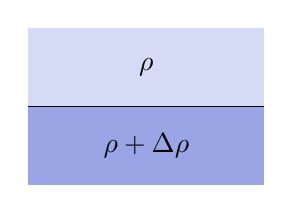
\begin{tikzpicture}
    \fill [mblue, opacity=0.5] (0, 0) rectangle (3, -1);
    \fill [mblue, opacity=0.2] (0, 0) rectangle (3, 1);

    \draw (0, 0) -- (3, 0);
    \node at (1.5, 0.5) {$\rho$};
    \node at (1.5, -0.5) {$\rho + \Delta \rho$};

  \end{tikzpicture}
\end{center}
However, if the interface is tilted, then there is a naturally induced torque:
\begin{center}
  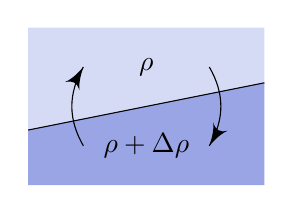
\begin{tikzpicture}
    \fill [mblue, opacity=0.5] (0, -0.3) -- (3, 0.3) -- (3, -1) -- (0, -1);
    \fill [mblue, opacity=0.2] (0, -0.3) -- (3, 0.3) -- (3, 1) -- (0, 1);

    \draw (0, -0.3) -- (3, 0.3);
    \node at (1.5, 0.5) {$\rho$};
    \node at (1.5, -0.5) {$\rho + \Delta \rho$};

    \draw (0.7, -0.5) edge [out=120, in=240, ->] (0.7, 0.5);
    \draw (2.3, 0.5) edge [out=300, in=60, ->] (2.3, -0.5);
  \end{tikzpicture}
\end{center}
In other words, \emph{vorticity} is induced. If we think about it, we see that the reason this happens is that the direction of the density gradient does not align with the direction of gravity. More precisely, this is because the density gradient does not align with the pressure gradient.

Let's try to see this from our equations. Recall that the vorticity is defined by\index{vorticity}\index{$\boldsymbol\omega$}
\[
  \boldsymbol\omega = \nabla \times \mathbf{u}.
\]
Taking the curl of the Navier--Stokes equation, and doing some vector calculus, we obtain the equation.
\[
  \frac{\partial \boldsymbol\omega}{\partial t} + \mathbf{u} \cdot \nabla \boldsymbol\omega = \boldsymbol\omega \cdot \nabla \mathbf{u} + \frac{1}{\rho^2}\nabla \rho \times \nabla P + \nu \nabla^2 \boldsymbol\omega
\]
The term on the left hand side is just the material derivative of the vorticity. So we should interpret the terms on the right-hand-side as the terms that contribute to the change in vorticity.

The first and last terms on the right are familiar terms that have nothing to do with the density gradient. The interesting term is the second one. This is what we just described --- whenever the pressure gradient and density gradient do not align, we have a \term{baroclinic torque}. % describe other terms as well.

%The left hand side is just the change in vorticity along the flow. The first term on the left is describing what happens when we stretch a vortex, which by conservation of momentum implies that the spin increases. The second term is what we just described --- if the pressure gradient points differently from the density gradient, then we get a torque, called \term{baroclinic torque}.

In general, equations are hard to solve, and we want to make approximations. A common approximation is the \term{Boussinesq approximation}. The idea is that even though the density difference is often what drives the motion, from the point of view of inertia, the variation in density is often small enough to be ignored. To take some actual, physical examples, salt water is roughly $4\%$ more dense than fresh water, and every $10$ degrees Celsius changes the density of air by approximately $4\%$.

Thus, what we do is that we assume that the density is constant except in the buoyancy force. The mathematically inclined people could think of this as taking the limit $g \to \infty$ but $\rho' \to 0$ with $g \rho'$ remaining finite.

Under this approximation, we can write our equations as
\begin{align*}
  \frac{\partial \mathbf{u}}{\partial t} + \mathbf{u}\cdot \nabla \mathbf{u} &= - \frac{1}{\rho_0} \nabla p' - g' \hat{\mathbf{z}} + \nu \nabla^2 \mathbf{u}\\
  \frac{\partial \boldsymbol\omega}{\partial t} + \mathbf{u} \cdot \nabla\boldsymbol\omega &= \omega \cdot \nabla \mathbf{u} + \frac{g}{\rho_0} \hat{\mathbf{z}} \times \nabla \rho + \nu \nabla^2 \boldsymbol\omega,
\end{align*}
where we define the \term{reduced gravity}  to be
\[
  g' = \frac{g \rho'}{\rho_0}
\]
Recall that our density is to be given by a function of temperature $T$. We must write down how we want the two to be related. In reality, this relation is extremely complicated, and may be affected by other external factors such as salinity (in the sea). However, we will use a ``leading-order'' approximation
\[
  \rho = \rho_0 (1 - \alpha(T - T_0)).
\]
We will also need to know how temperature $T$ evolves in time. This is simply given by the diffusion equation
\[
  \frac{\partial T}{\partial t} + \mathbf{u} \cdot \nabla T = \kappa \nabla^2 T.
\]
Note that in thermodynamics, temperature and pressure are related quantities. In our model, we will completely forget about this. The only purpose of pressure will be to act as a non-local Lagrange multiplier that enforces incompressibility.

There are some subtleties with this approximation. Inverting the relation,
\[
  T = \frac{1}{\alpha}\left(1 - \frac{\rho}{\rho_0}\right) + T_0.
\]
Plugging this into the diffusion equation, we obtain
\[
  \frac{\partial \rho}{\partial t} + \mathbf{u} \cdot \nabla \rho = \kappa \nabla^2 \rho.
\]
The left-hand side is the material derivative of density. So this equation is saying that density, or mass, can ``diffuse'' along the fluid, independent of fluid motion. Mathematically, this follows from the fact that density is directly related to temperature, and temperature diffuses.

This seems to contradict the conservation of msas. Recall that the conservation of mass says
\[
  \frac{\partial \rho}{\partial t} + \nabla \cdot (\mathbf{u} \rho) = 0.
\]
We can than expand this to say
\[
  \frac{\partial \rho}{\partial t} + \mathbf{u} \cdot \nabla \rho = - \rho \nabla \cdot \mathbf{u}.
\]
We just saw that the left-hand side is given by $\kappa \nabla^2 \rho$, which can certainly be non-zero, but the right-hand side should vanish by incompressibility! The issue is that here the change in $\rho$ is not due to compressing the fluid, but simply thermal diffusion.

If we are not careful, we may run into inconsistencies if we require $\nabla \cdot \mathbf{u} = 0$. For our purposes, we will not worry about this too much, as we will not use the conservation of mass.

We can now return to our original problem. We have a fluid of viscosity $\nu$ and thermal diffusivity $\kappa$. There are two plates a distance $d$ apart, with the top held at temperature $T_0$ and bottom at $T_0 + \Delta T$. We make the Boussinesq approximation.
\begin{center}
  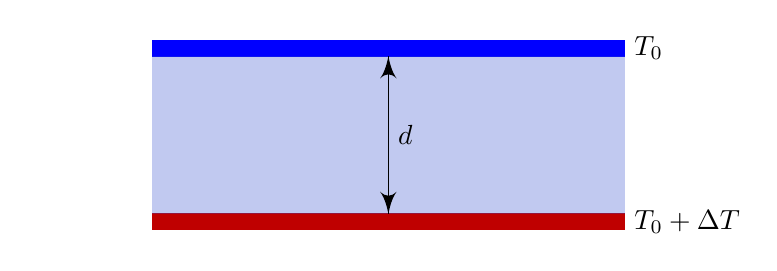
\begin{tikzpicture}
    \draw [red!50!mred, fill] (0, 0) rectangle (6, -0.2);
    \draw [blue, fill] (0, 2) rectangle (6, 2.2);

    \fill [mblue, opacity=0.3] (0, 0) rectangle (6, 2);

    \node [right] at (6, 2.1) {$T_0$};
    \node [right] at (6, -0.1) {$T_0 + \Delta T$};
    \node [white, left] at (0, -0.1) {$T_0 + \Delta T$};

    \draw [<->] (3, 0) -- (3, 2) node [pos=0.5, right] {$d$};
  \end{tikzpicture}
\end{center}
We first solve for our steady state, which is simply
\begin{align*}
 U &= 0\\
 T_h &= T_0 - \Delta T \frac{(z - d)}{d}\\
 \rho_h &= \rho_0 \left(1 + \alpha \Delta T \frac{z - d}{d}\right)\\
 P_h &= P_0 - g \rho_0 \left(z + \frac{\alpha \Delta Tz}{2d}(z - 2d)\right),
\end{align*}
In this state, the only mode of heat transfer is conduction. What we would like to investigate, of course, is whether this state is stable. Consider small perturbations
\begin{align*}
  \mathbf{u} &= \mathbf{U} + \mathbf{u}'\\
  T &= T_h + \theta\\
  P &= P_h + p'.
\end{align*}
We substitute these into the Navier--Stokes equation. Starting with
\[
  \frac{\partial \mathbf{u}}{\partial t} + \mathbf{u} \cdot \nabla \mathbf{u} = -\frac{1}{\rho_0} \nabla p' + g \alpha \theta \hat{\mathbf{z}} + \nu \nabla^2 \mathbf{u},
\]
we assume the term $\mathbf{u} \cdot \nabla \mathbf{u}$ will be small, and end up with the equation
\[
  \frac{\partial \mathbf{u}'}{\partial t} = - \frac{1}{\rho_0} \nabla p' + g \alpha \theta \hat{\mathbf{z}} + \nu \nabla^2 \mathbf{u},
\]
together with the incompressibility condition $\nabla \cdot \mathbf{u}' = 0$.

Similarly, plugging these into the temperature diffusion equation gives us
\[
  \frac{\partial \theta}{\partial t} - w' \frac{\Delta T}{d} = \kappa \nabla^2 \theta,
\]
where $w$ is the velocity in the $z$ direction.

We can gain further understanding of these equations by expressing them in terms of dimensionless quantities. We introduce new variables
\begin{align*}
  \tilde{t} &= \frac{\kappa t}{d^2} & \tilde{\mathbf{x}} &= \frac{\mathbf{x}}{d}\\
  \tilde{\theta} &= \frac{\theta}{\Delta T} & \tilde{p} &= \frac{d^2 p'}{\rho_0 \kappa^2}
\end{align*}
In terms of these new variables, our equations of motion become rather elegant:
\begin{align*}
  \frac{\partial \tilde{\theta}}{\partial \tilde{t}} - \tilde{w} &= \tilde{\nabla}^2 \tilde{\theta}\\
  \frac{\partial \tilde{\mathbf{u}}}{\partial \tilde{t}} &= - \tilde{\nabla} \tilde{p} + \left(\frac{g\alpha \Delta T d^3}{\nu\kappa}\right) \left(\frac{\nu}{\kappa}\right) \tilde{\theta} \hat{\mathbf{z}} + \frac{\nu}{\kappa} \tilde{\nabla}^2 \tilde{\mathbf{u}}
\end{align*}
Ultimately, we see that the equations of motion depend on two dimensionless constants: the \term{Rayleigh number} and \term{Prandtl number}
\begin{align*}
  \Ra &= \frac{g\alpha \Delta T d^3}{\nu\kappa}\\
  \Pr &= \frac{\nu}{\kappa},
\end{align*}
These are the two parameters control the behaviour of the system. In particular, the Prandtl number measures exactly the competition between viscous and diffusion forces. Different fluids have different Prandtl numbers:
\begin{itemize}
  \item In a gas, then $\frac{\nu}{\kappa} \sim 1$, since both are affected by the mean free path of a particle.
  \item In a non-metallic liquid, the diffusion of heat is usually much slower than that of momentum, so $\Pr \sim 10$.
  \item In a liquid metal, $\Pr$ is very very low, since, as we know, metal transmits heat quite well.
\end{itemize}
Finally, the incompressibility equation still reads
\[
  \tilde{\nabla} \cdot \tilde{\mathbf{u}} = 0
\]
Let's start with some rather vague analysis of stability. 

It is normal to expect that if $\Delta T$ is large, then the system is unstable. But in $\Ra$, we see that we should compare $\Delta T$ to $\Ra$. Why is this the case?

The reason convection happens is that we want to convert the potential energy of the liquid into kinetic energy by moving the lighter liquid to the top. There are two factors that try to stop this. The first is that there is some viscosity resiting the motion, and the other is that the very essense that is leading to the motion is itself diffusing through the fluid already.

More mathematically, if we move some $d \times d \times d$ block of liquid from the bottom to the top, the potential energy released is $gd (\Delta \rho d^3) \sim g \rho_0 \alpha \Delta T d^4$. The time scale for this to happen is $\tau \sim d/U$. % in a d x d x d cell

On the other hand, the heat is diffused away on a time sacle of $\tau \sim d^2 /\kappa$. Thus, we find that $U \sim \kappa/d$.

The viscous stress is $\mu \frac{\partial u}{\partial z} \sim \frac{\mu U}{d}$, and so the force is the integral over the area, so it is $\sim \frac{\mu U}{d} d^2$. Then the work done is $\int F \d z$, and so is $\frac{\mu U}{d} d^2 d$.

So there is enough potential energy to ``pay'' for the motion of PE $>$ W, i.e.
\[
  g \rho_0 \alpha \Delta T d^4 \gtrsim \rho_0 \nu \kappa d,
\]
and so we need
\[
  \Ra = \frac{g \alpha \Delta T d^3}{\nu \kappa} = \frac{g' d^3}{\nu \kappa} \gtrsim 1.
\]
Let's now do this properly. Taking the curl of the Navier--Stokes equation, and dropping the tildes, we obtain
\[
 \frac{\partial \boldsymbol\omega}{\partial t} = \Ra \Pr \nabla \theta \times \hat{\mathbf{z}} + \Pr \nabla^2 \boldsymbol\omega
\]
Recall our temperature equation is
\[
  \frac{\partial \theta}{\partial t} - w = \nabla^2 \theta.
\]
To connect these two together, we take the curl of the first equation again, to obtain
\[
 \frac{\partial}{\partial t} \nabla^2 \mathbf{u} = \Ra \Pr \left(\nabla^2 \theta \hat{\mathbf{z}} - \nabla \left(\frac{\partial \theta}{\partial z}\right)\right) + \Pr \nabla^4 \mathbf{u}
 \]
% w is the z component of u!
Combining our equations and taking the $z$ component, we have
\[
  \frac{\partial}{\partial t} \nabla^2 w = \Ra \Pr \left(\frac{\partial^2}{\partial x^2} + \frac{\partial^2}{\partial y^2}\right) \theta + \Pr \Delta^4 w.
\]
We note that this is in fact a $6$th order differential equation in space, so we need to impose $6$ boundary conditions, imposed at $z =0 , 1$. Reasonable conditions include
\begin{itemize}
  \item $w = 0 = \theta$ at the boundary, imposing impermeable boundaries
\end{itemize}
It is also \emph{convenient} to assume the top and bottom surfaces are stress-free: $\frac{\partial u}{\partial z} = \frac{\partial v}{\partial z} = 0$, which implies
\[
  \frac{\partial}{\partial z} \left(\frac{\partial u}{\partial x} + \frac{\partial v}{\partial y}\right) = 0.
\]
This then gives us $\frac{\partial^2 w}{\partial z^2} = 0$. This is does \emph{not} make much physical sense, because our fluid is viscous, and we should expect no-slip boundary conditions, not no-stress. But they are mathematically convenient, and we shall assume them.

We can now use separation of variables. We see that the equations are symmetric in $x$ and $y$, and so we write our solution as
\begin{align*}
  w &= W(z) X(x, y) e^{\sigma t}\\
  \theta &= \Theta(z) X(x, y) e^{\sigma t}.
\end{align*}
We can rewrite our temperature equation as
\[
  \left(\frac{\d^2}{\d z^2} - \sigma + \left(\frac{\partial^2}{\partial x^2} + \frac{\partial^2}{\partial y^2}\right)\right) X \Theta = -XW.
\]
Or equivalently
\[
  \left(\frac{\d^2}{\d z^2} - \sigma\right) X\Theta + XW = - \left(\frac{\partial^2}{\partial x^2} + \frac{\partial^2}{\partial y^2}\right) X\Theta.
\]
We see that the the differential operator on the left only acts in $\Theta$, while those on the right only act on $X$. So we can perform our classic separation of variables, writing the equation as
\[
  \frac{\left(\frac{\d^2}{\d y^2} - \sigma\right) \Theta + W}{\Theta} = - \frac{\left(\frac{\d^2}{\d x^2} + \frac{\d^2}{\d y^2}\right) X}{X}.
\]
Since the LHS is purely a function of $z$, and the RHS is purely a function of $X$, they must be constant, and by requiring that the solution is bounded, we see that this contant must be positive. Our equations then become
\begin{align*}
  \left(\frac{\partial^2}{\partial x^2} + \frac{\partial^2}{\partial y^2} \right)X = - \lambda^2 X\\
  \left(\frac{\d^2}{\d z^2} - \lambda^2 - \sigma\right) \Theta = - W.
\end{align*}
We now look at our other equation. Plugging in our expressions for $w$ and $\theta$, and using what we just obtained, we have
\[
  \sigma\left(\frac{\d^2}{\d z^2} - \lambda^2 \right)W = - \Ra \Pr \lambda^2 \Theta + \Pr \left(\frac{\d^2}{\d z^2} - \lambda^2\right)^2 W.
\]
On the boundary, we have $\Theta = 0$, and also $W$ and $\frac{\partial^2}{\partial z^2}W = 0$, by assumption. So it follows that we must
\[
  \left.\frac{\d^4}{\d z^4}W \right|_{z = 0, 1} = 0.
\]
We can eliminate $\Theta$ by letting $\left(\frac{\d^2}{\d z^2} - \sigma - \lambda^2\right)$ act on both sides, which convertes th $\Theta$ into $W$. We are then left with a $6$th order differential equation
\[
  \left(\frac{\d^2}{\d z^2} - \sigma - \lambda^2\right) \left(\Pr \left(\frac{\d^2}{\d z^2} - \lambda^2\right)^2 - \sigma \left(\frac{\d^2}{\d z^2} - \lambda^2\right)\right) W =- \Ra \Pr \lambda^2 W.
\]
This is an eigenvalue problem, and we see that our operator is self-adjoint. We can factorize and divide across by $\Pr$ to obtain
\[
  \left(\frac{\d^2}{\d z^2} - \lambda^2 \right) \left(\frac{\d^2}{\d z^2} - \sigma - \lambda^2\right) \left(\frac{\d^2}{\d z^2} - \lambda ^2 - \frac{\sigma}{\Pr}\right) W = - \Ra \lambda^2 W.
\]
The boundary conditions are that
\[
  W= \frac{\d^2 W}{\d z^2}= \frac{\d^4 W}{\d x^4} = 0\text{ at }z = 0, 1.
\]
We see that any eigenfunction of $\frac{\d^2}{\d z^2}$ gives us an eigenfunction of our big scary differential operator, and our solutions are quantized sine functions, $W = \sin n \pi z$ with $n \in \N$. In this case, the eigenvalue equation is
\[
  \Ra \lambda^2 = (n^2 \pi^2 + \lambda^2) (n^2 \pi^2 + \sigma + \lambda^2) \left(n^2\pi^2 + \lambda^2 + \frac{\sigma}{\Pr}\right) = \Ra \lambda^2.
\]
This is a quadratic function of $\sigma$, so we can explicitly write out the growth rates.

The interesting bit is that the marginal stability condition is $\sigma = 0$. And in this case, $\Pr$ drops out of the equation. So regardless of what fluid we are using, we find that the Critical Rayleigh number is
\[
  \Ra_c(n) = \frac{(n^2 \pi^2 + \lambda^2)^3}{\lambda^2},
\]
and the smallest such value is obtained when $n = 1$. We can then minimize $\lambda^2$, setting
\[
  0 = \frac{\d \Ra_c(1)}{\d [\lambda^2]} = \frac{(\pi^2 + \lambda^2)^2}{\lambda^4}(2\lambda^2 - \pi^2).
\]
So we find that we need
\[
  \lambda_c = \frac{\pi}{\sqrt{2}}.
\]
So we find that
\[
  \Ra_c = \frac{27\pi^4}{4} \approx 657.5.
\]
So for small $\Ra_c$, all modes are stable, and as $\Ra$ increases, the range of unstable mode increases.

% insert picture

In general, the critiacal $\Ra$ depends on the boundary condition, the picture is rather generic, with the width of the unstable regime grows as $\sqrt{\Ra - \Ra_c}$.

We might ask --- how does convection enhance the heat flux? This is quantified by the \term{Nusselt number}
\[
  Nu = \frac{\text{convective heat transfer}}{\text{conductive heat transfer}} = \frac{\bra wT\ket d}{\kappa \Delta T} = \bra \tilde{w} \tilde{\theta}.
\]
Since this is a non-dimensional number, we know it is a function of $\Ra$ and $\Pr$.

There is some simple arguments we can make about this. If we have a purely conductive state, then we expecet the temperature gradient to look like this:
\begin{center}
  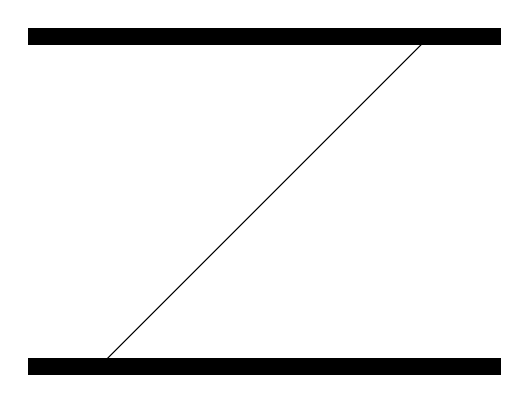
\begin{tikzpicture}
    \draw [fill] (0, 0) rectangle (6, -0.2);
    \draw [fill] (0, 4) rectangle (6, 4.2);

    \draw (1, 0) -- (5, 4);
  \end{tikzpicture}
\end{center}
But in reality, because on convection, it looks more like this:
\begin{center}
  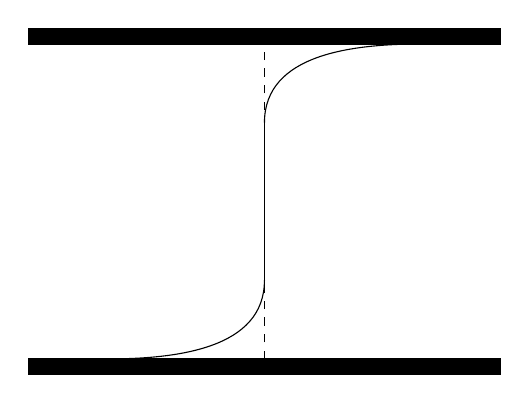
\begin{tikzpicture}
    \draw [fill] (0, 0) rectangle (6, -0.2);
    \draw [fill] (0, 4) rectangle (6, 4.2);

    \draw (1, 0) edge [out=0, in=270] (3, 1);
    \draw (3, 1) -- (3, 3) edge [out=90, in=180] (5, 4);

    \draw [dashed] (3, 0) -- (3, 4);
  \end{tikzpicture}
\end{center}
The idea is that near the boundary layer, once we have things of sufficiently large/small temperature, convection kicks in and sends the parcel off to the other side.

Based on this model, the convective heat transfer should be independent of layer depth, because the boundary layer only needs to shoot the hot parcels off, and doesn't really care where it goes. So $\bra wT \ket \propto d^0$. So $Nu \propto d$, and hence it must depend on $\Ra$ as $Nu \propto \Ra^{1/3}$.

Of course, the real situation is much more subtle.

\subsection{Classical Kelvin--Helmholtz instability}
Let's now look at classical Kelvin--Helmholtz instability. This is similar to Rayleigh--Taylor instability, but we consider the case where there is in fact flow in the two layers. We can still use a velocity potential
\[
  (u, w) = \left(\frac{\partial \phi}{\partial x}, \frac{\partial \phi}{\partial z}\right).
\]
We shall only consider the system in $2D$. The far field now has velocity
\begin{align*}
  \phi_1 &= U_1 x + \phi_1'\\
  \phi_2 &= U_2 x + \phi_2'
\end{align*}
with $\phi_1' \to 0$ as $z \to \infty$ and $\phi_2' \to 0$ as $z \to -\infty$.

The boundary conditions are the same. Continuity of vertical velocity requires
\[
  \left.\frac{\partial \phi_{1, 2}}{\partial z} \right|_{z = \eta} = \frac{\D \eta}{\D t}.
\]
The dynamic boundary condition is that we have continuity of pressure at the interface if there is no surface tension, in which case Bernoulli tells us
\[
  \rho_1 \frac{\partial \phi_1}{\partial t} + \frac{1}{2} \rho_1 |\nabla \phi_1|^2 + g \rho_1 \eta = \rho_2 \frac{\partial \phi_2}{\partial t} + \frac{1}{2} \rho_2 |\nabla \phi_2|^2 + g \rho_2 \eta.
\]
The interface conditions are non-linear, and again we want to linearize. But since $U_{1, 2}$ is of order $1$, linearization will be different. We have
\[
  \left. \frac{\partial \phi'_{1, 2}}{\partial z} \right|_{z = 0} = \left(\frac{\partial}{\partial t} + U_{1, 2} \frac{\partial}{\partial x}\right)\eta.
\]
So the Bernoulli condition gives us
\[
  \rho_1 \left(\left(\frac{\partial}{\partial t} + U_1 \frac{\partial}{\partial x}\right) \phi_1' + g \eta\right) = \rho_2 \left(\left(\frac{\partial}{\partial t} + U_2 \frac{\partial}{\partial x}\right) \phi_2' + g \eta\right)
\]
This modifies our previous eigenvalue problem for the phase speed and wavenumber $\omega = k c$, $k = \frac{2\pi}{\lambda}$. We go exactly as before, and after some work, we find that we have
\[
  c = \frac{\rho_1 U_1 + \rho_2 U_2}{\rho_1 + \rho_2} \pm \frac{1}{\rho_1 + \rho_2} \left(\frac{g (\rho_2^2 - \rho_1^2)}{k} - \rho_1 \rho_2 (U_1 - U_2)^2\right)^{1/2}.
\]
So we see that we have instability if $c$ has an imaginary part, i.e.
\[
  k > \frac{g (\rho_2^2 - \rho_1^2}{\rho_1 \rho_2 (U_1 - U_2)^2}.
\]
So we see that there is instability for sufficiently large wavenumbers, even for static stability. Similar to Rayleigh--Taylor instability, the growth rate $k c_i$ grows monotonically with wavenumber, and as $k \to \infty$, the instability becomes proportional to the difference $|U_1 - U_2|$ (as opposed to Rayleigh--Taylor instability, where it is infinite). % c_i and c_r are real and imaginary components of c

One way to think about this is that if $U_1 \not= U_2$, then at the boundary, there is a $\delta$-function of vorticity, which is highly unstable! By practically, this is of course not the case. 

By changing the frame of reference, we can wlog assume $U_1 = U = - U_2$. In the Boussinesq limit,  we have $c_r = 0$ and have instability for $\frac{g \Delta \rho \lambda}{\rho U^2} < 4\pi$. We can see the numerator as the potential energy cost if we move a parcel from the bottom layer to the top layer, while the denominator as some sort of kinetic energy. So this says we are unstable if there is enough kinetic energy to move a parcel up.

There are some important outstanding questions:
\begin{itemize}
  \item How might we regularize this expression? The vortex sheet is obviously wildly unstable
  \item Was it right to assume two-dimensional perturbations?
  \item What happens if we regularize the depth of the shear?
\end{itemize}

We first look at what happens when we work in $3$ dimensions. The inviscid homogeneous incompressible Navier--Stokes equations are again
\[
  \left(\frac{\partial \mathbf{u}}{\partial t} + \mathbf{u} + \mathbf{u} \cdot \nabla \mathbf{u}\right) = \frac{\D \mathbf{u}}{\D t} = - \nabla \left(\frac{p'}{\rho}\right),\quad \nabla \cdot \mathbf{u} = 0.
\]
We linearize about a shear flow, and consider some 3D normal modes
\[
  \mathbf{u} = \bar{U}(z)\hat{\mathbf{x}} + \mathbf{u}'(x, y, z, t),
\]
where
\[
  (\mathbf{u}', p'/\rho) = [\hat{\mathbf{u}}(z), \hat{p}(z)]e^{i (kx + \ell y - kct)}.
\]
Here the average flow goes in the direction of $\hat{\mathbf{x}}$, but we allow our perturbation to point at an angle. The phase speed is
\[
  c_p = \frac{\omega}{\kappa} = \frac{\omega}{(k^2 + \ell^2)^{1/2}} = \frac{kc_r}{(k^2 + \ell^2)^{1/2}}
\]
and the growth rate is $\sigma_{3d} = k c_i$.

We substitute this into the equations to obtain
\begin{align*}
  ik (\bar{U} - c) \hat{u} + \hat{w} \frac{\d}{\d z} \bar{U} &= - ik \hat{p}\\
  ik (\bar{u} - c) \hat{v} &= - il \hat{p}\\
  ik (\bar{u} - c) \hat{w} &= - \frac{\d}{\d z} \hat{p}\\
  ik \hat{u} + i\ell\hat{v} + \frac{\d}{\d z} \hat{w} &= 0
\end{align*}
We can rearrange the first three equations and do nothing to the last to get
\begin{align*}
  ik (\bar{U} - c) \hat{u} + \hat{w} \frac{\d}{\d z} \bar{U} &= - iki^2 \frac{\hat{p}}{k}\\
  i\ell (\bar{u} - c) \hat{v} &= - i\ell^2 \frac{\hat{p}}{k}\\
  ik (\bar{u} - c) \hat{w} &= - \frac{\d}{\d z} \hat{p}\\
  ik \hat{u} + i\ell\hat{v} + \frac{\d}{\d z} \hat{w} &= 0
\end{align*}
We see that the equations naturally group into terms involving $k\hat{u} \ell \hat{v}$. We can get
\[
  i(\bar{U} - c) (k \hat{u} + \ell\hat{v}) + \hat{w} \frac{\d}{\d z} \bar{U} = - i\kappa \left(\frac{\kappa \hat{p}}{k}\right)
\]
We introduce new variables
\[
  \kappa \tilde{u} + k \hat{u} \ell \hat{v},\quad \tilde{p} = \frac{\kappa \hat{p}}{k}.
\]
So we have equations
\begin{align*}
  i (\bar{U} - c) \kappa \tilde{u} + \hat{w} \frac{\d \bar{U}}{\d z} &= - i \kappa \tilde{p}\\
  i \kappa (\bar{U} - c) \hat{w} = - \frac{\d}{\d z} \tilde{p}\\
  \kappa \tilde{U} + \frac{\d \hat{w}}{\d z} &= 0.
\end{align*}
This looks just like a $2d$ system. So the $3d$ problem has an equivalent 2d problem with $\sigma_{2d} = \kappa c_i > k c_i = \sigma_{3d}$. This is Squire's Theorem.

One way to think about this is that the $y$ component of the perturbation sees less of the original velocity $\bar{U}$, and so it is more stable.

So we restrict attention to two-dimensional perturbations, and so
\begin{align*}
  ik (\bar{U} - c) \hat{u} + \hat{w} \frac{\d}{\d z} \bar{U} &=  ik\hat{p}\\
  ik (\bar{U} - c) \hat{w} &= - \frac{\d}{\d z} \hat{p}\\
  ik \hat{u} + \frac{\d}{\d z} \hat{w} &= 0.
\end{align*}
We use incompressibility to eliminate $y$ from the first equation, and we are left with
\[
  -(\bar{U} - c) \frac{\d}{\d z} \hat{w} + \hat{w} \frac{\d}{\d z} \bar{U} = - ik \hat{p} 
\]
Differentiating with respect to $z$ gives us
\[
  -(\bar{U} - c) \frac{\d^2}{\d z^2} \hat{w} - \frac{\d}{\d z} \hat{w} \frac{\d}{\d z} \bar{U} + \frac{\d}{\d z} \hat{w} \frac{\d}{\d z} \bar{U} + \hat{w} \frac{\d^2}{\d z^2} \bar{U} = -k^2 (\bar{U} - c) \hat{w}.
\]
The terms in the middle cancel, and we can rearrange to obtain the \term{Rayleigh equation}
\[
  \left((\bar{U} - c) \left(\frac{\d^2}{\d z^2} - k^2\right) - \frac{\d^2}{\d z^2} \bar{U} \right)  \hat{w} = 0.
\]
We see that when $\bar{U} = c$, we have a regular singular point.

We can express this in terms of a streamfunction $\boldsymbol\Psi$, defined by
\[
  \nabla \times \boldsymbol\Psi = \mathbf{u}'.
\]
Writing $\boldsymbol\Psi = (0, \psi ,0)$, we have
\[
  - \frac{\partial \psi}{\partial z} = u',\quad \frac{\partial \psi}{\partial x} = w'.
\]
So we have
\[
  \frac{\d \hat{\psi}}{\d z} = \hat{u},\quad ik \hat{\psi} = \hat{w}.
\]
The natural boundary conditions are that $\hat{w} \to 0$ at the edge of the domain.

But note that this differential operator is not self-adjoint! This is since $\bar{U}$ has non-trivial $z$-dependence. This means we do not have a complete basis of orthogonal eigenfunctions. This is manifested by the fact that it can have transient growth.

Now we may wlog $-L < z < L$, and then rewrite Rayleigh equation in conventional form:
\[
  \frac{\d^2 \hat{w}}{\d z^2} - k^2 \hat{w} - \frac{\frac{\d^2j\d z^2}{\bar{U}}}{\bar{U} - c} \hat{w} = 0.
\]
We multiply by $w^*$, integrate across the domain, and apply boundary conditions to obtain
\[
  \int_{-L}^L \frac{\bar{U}''}{\bar{U} - c} |\hat{w}|^2 \;\d z = - \int_{-L}^L (|\hat{w}'|^2 + k^2 |\hat{w}|^2)\;\d z
\]
We can split the LHS into real and imaginary parts:
\[
  \int_{-L}^L \left( \frac{\bar{U}''(\bar{U} - c_r)}{|\bar{U} - c|^2}\right) |\hat{w}|^2 \;\d z + i c_i \int_{-L}^L \left(\frac{\bar{U}''}{ |\bar{U} - c|^2}\right) |\hat{w}|^2 \;\d z.
\]
But since the RHS is purely real, we know the imaginary part must vanish.

One way for the imaginary part to vanish is for $c_i$ to vanish, and this corresponds to stable flow. If we want $c_i$ to be non-zero, then the integral must vanish. So we obtain the \term{Rayleigh inflection point criterion}: $\frac{\d^2}{\d z^2} \bar{U}$ must change sign at least once in $-L < z < L$.

The real part shows that this condition is not sufficient. We need something to ensure that the real integral is negative as well. This was noticed by Fjortoft.

We define $z_s, \bar{U}_s = \bar{z_s}, \bar{U}''(z_s) = 0$, i.e. the location and velocity at the inflection part.

For instability to exist, we require that $\int_{-L}^L \left(\frac{\bar{U}''}{|\bar{U} - c|^2} \right) |\hat{w}|^2\;\d z$ must vanish. So we can add $(c_r - \bar{U}_s)\int_{-L}^L \left(\frac{\bar{U}''}{|\bar{U} - c|^2} \right) |\hat{w}|^2\;\d z$ to the right hand side to obtain
\[
  -\int_{-L}^L (|\hat{w}'|^2 + k^2 |\hat{w}|^2)\;\d z = \int_{-L}^L \left(\frac{\bar{U}''(\bar{U} - \bar{U}_s)}{ |\bar{U} - c|^2} \right) |\hat{w}|^2\;\d z.
\]
Suppose $\bar{U}$ is monotone and has one inflection point in $-L < L$. Then we must have that $\bar{U}'' (\bar{U} - \bar{U_s}) \leq 0$ with equality only at $z$.

% insert examples


\printindex
\end{document}
